\sloppy
\chapter{Proposed Approach}
\addtocontents{toc}{\protect\setcounter{tocdepth}{2}}
\section{Introduction}

This chapter describes the fake news detection system proposed and evaluated in this thesis. It begins with a formal problem statement, then presents the overall system model as an end-to-end pipeline, followed by a detailed description of the proposed BERT + BiLSTM classification architecture, the underlying algorithm, and the design rationale for combining a transformer encoder with a sequential BiLSTM layer.

\section{Problem Statement}

Given a piece of news text $T$ (an article body, headline, or short statement), the goal is to learn a classification function $f(T) \rightarrow \{\text{REAL}, \text{FAKE}\}$ that predicts whether $T$ represents genuine or fabricated/misleading news, along with an associated confidence score. The function $f$ must be learned from labelled training data drawn from one or more benchmark datasets, and must generalize not only to unseen examples from the same dataset, but ideally also across datasets with different sources, writing styles, and label distributions (evaluated in this thesis using LIAR and ISOT, as discussed in Chapter~5).

This thesis specifically investigates three candidate realizations of $f$: a purely sequential deep learning model (BiLSTM), a purely transformer-based model (BERT), and a hybrid model that composes both (BERT + BiLSTM), with the aim of empirically determining which realization offers the best trade-off between detection accuracy, generalization across datasets, and model complexity.

\section{System Model}

The proposed detection system is designed as a multi-stage pipeline that converts unstructured news input into a classified output with an associated confidence estimate. Figure~\ref{fig:systemmodel} illustrates the overall system architecture.

\begin{figure}[H]
    \centering
    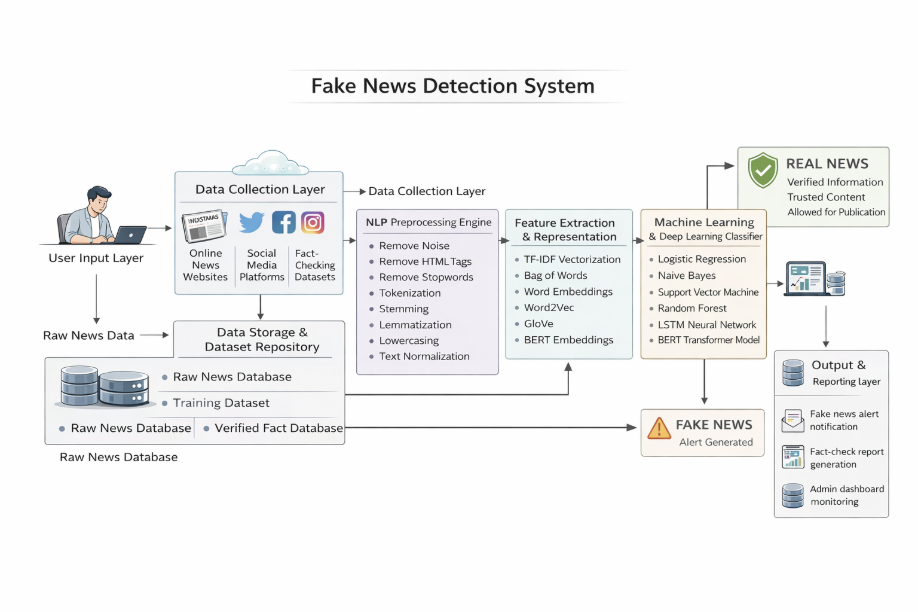
\includegraphics[width=0.95\textwidth]{architecture.png}
    \caption{End-to-end fake news detection system pipeline, from user input through data collection, NLP preprocessing, feature extraction, classification, and output reporting}
    \label{fig:systemmodel}
\end{figure}

The pipeline is organized into the following stages:

\begin{itemize}
\item \textbf{User Input Layer:} Accepts raw news input in the form of free text, a headline, or a URL pointing to a news article.
\item \textbf{Data Collection Layer:} Gathers the corresponding data from benchmark datasets (LIAR, ISOT, FakeNewsNet) and, where applicable, online news websites, social media platforms, and fact-checking sources.
\item \textbf{Data Storage and Dataset Repository:} Persists raw news data, training/validation/test splits, and verified fact databases for reuse across experiments.
\item \textbf{NLP Preprocessing Engine:} Cleans and normalizes the raw text through noise removal, HTML-tag stripping, stopword removal, tokenization, stemming, lemmatization, and lowercasing, as detailed in Chapter~2.
\item \textbf{Feature Extraction and Representation Layer:} Converts the normalized text into numeric representations using TF-IDF, Bag-of-Words, Word2Vec, GloVe, and/or BERT embeddings, depending on the downstream classifier.
\item \textbf{Machine Learning and Deep Learning Classifier:} Hosts the candidate classification models compared in this thesis -- BiLSTM, BERT, and the hybrid BERT + BiLSTM model -- and produces a REAL/FAKE prediction with a confidence score.
\item \textbf{Output and Reporting Layer:} Emits the final classification decision together with a human-readable report, suitable for downstream use cases such as a fake-news alert notification, a fact-check report, or an administrative monitoring dashboard.
\end{itemize}

This layered design cleanly separates preprocessing, representation, and modelling concerns, which makes it straightforward to swap in the different classifiers evaluated in Chapter~5 (BiLSTM, BERT, BERT + BiLSTM) without changing the surrounding pipeline.

\section{Proposed BERT + BiLSTM Detection Framework}

While the system model in Figure~\ref{fig:systemmodel} shows the pipeline at a high level, Figure~\ref{fig:architecture} zooms into the detailed architecture of the best-performing classifier evaluated in this thesis: the hybrid BERT + BiLSTM model.

\begin{figure}[H]
    \centering
    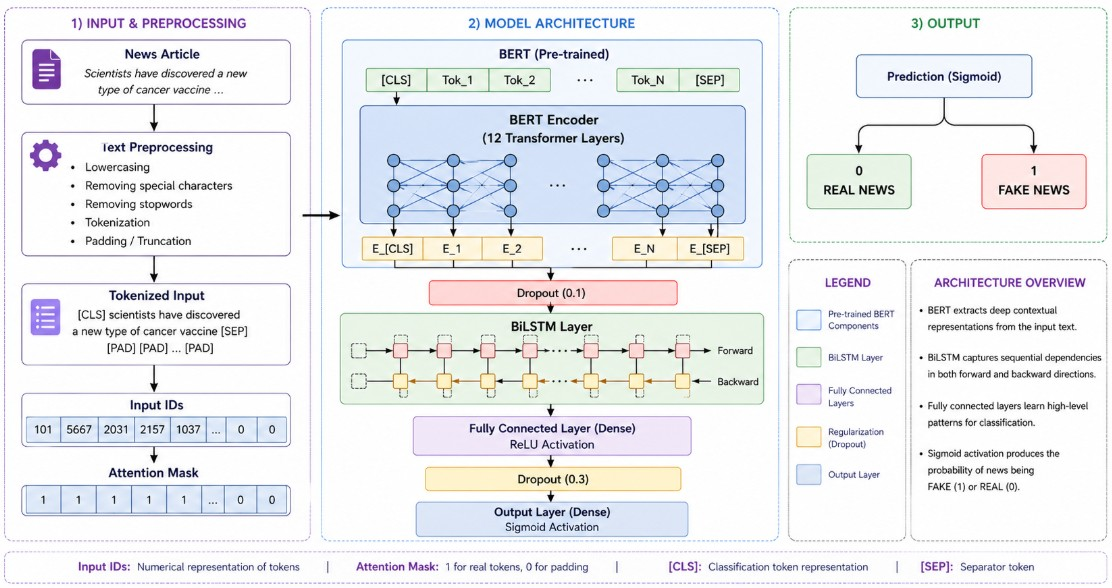
\includegraphics[scale=0.6]{Arch.jpg}
    \caption{Detailed architecture of the proposed BERT + BiLSTM fake news detection model}
    \label{fig:architecture}
\end{figure}

As shown in the figure, the input news article is first tokenized and normalized (lowercasing, special-character removal, stopword removal, tokenization, padding/truncation), producing a fixed-length sequence of token IDs together with an attention mask. This tokenized sequence, prefixed with a \texttt{[CLS]} token and suffixed with a \texttt{[SEP]} token, is passed through a pre-trained BERT encoder consisting of 12 Transformer layers, which produces a contextual embedding for every token position ($E_{[CLS]}, E_1, \ldots, E_N, E_{[SEP]}$).

Rather than discarding all but the \texttt{[CLS]} embedding, as is common in simple BERT fine-tuning setups, the proposed model passes the entire sequence of contextual embeddings through a dropout layer (rate 0.1) and then into a BiLSTM layer, which processes the sequence in both forward and backward directions to capture sequential dependencies over BERT's already-contextualized representations. The output of the BiLSTM layer is passed through a fully connected (dense) layer with a ReLU activation, followed by a second dropout layer (rate 0.3), and finally an output dense layer with a sigmoid activation that produces the probability of the input being fake (1) or real (0).

\subsection{Proposed Algorithm}

The complete classification procedure for the proposed BERT + BiLSTM model is summarized in Algorithm~\ref{alg:bertbilstm}.

\begin{algorithm}[H]
\SetAlgoLined
\KwIn{Raw news text $T$}
\KwOut{Classification label $y \in \{\text{REAL}, \text{FAKE}\}$ with confidence score}
Preprocess $T$: apply noise removal, lowercasing, tokenization, stopword removal, and lemmatization\;
Tokenize the preprocessed text using BERT's WordPiece tokenizer, prepend \texttt{[CLS]} and append \texttt{[SEP]}\;
Pass the tokenized sequence through the pre-trained BERT encoder to obtain contextual embeddings $E_{[CLS]}, E_1, \ldots, E_N, E_{[SEP]}$\;
Apply dropout to the sequence of contextual embeddings\;
Pass the embedding sequence through a BiLSTM layer to obtain sequence-aware hidden representations\;
Pass the BiLSTM output through a fully connected layer with ReLU activation\;
Apply dropout, then pass the result through an output dense layer with sigmoid activation\;
\Return{predicted label $y$ (REAL or FAKE) and its associated confidence score}\;
\caption{Fake News Detection using the Proposed BERT + BiLSTM Model}
\label{alg:bertbilstm}
\end{algorithm}

\subsection{Design Rationale: Why Combine BERT and BiLSTM?}

It is worth emphasizing that the motivation for combining BERT and BiLSTM is not that BiLSTM performs poorly on its own (although, as shown in Chapter~5, it does under the training conditions used in this thesis). Rather, the two model families have complementary strengths that motivate the hybrid design explored here. BERT excels at capturing context and semantics within text through its bidirectional Transformer design and self-attention mechanism, but its primary mechanism for aggregating sequence-level information is attention rather than explicit sequence modelling of the kind performed by recurrent networks.

BiLSTM, on the other hand, is purpose-built for modelling sequences and capturing temporal/positional dependencies in text, processing its input in both forward and backward directions. In the proposed hybrid framework, BERT acts as a contextual feature extractor that produces informative token-level embeddings; rather than depending solely on the \texttt{[CLS]} token, the entire sequence of contextual embeddings generated by BERT is fed into the BiLSTM layer, allowing the network to layer explicit sequential modelling on top of BERT's already rich contextual representations.

Consequently, the resulting BERT + BiLSTM framework is designed to benefit from both contextual embeddings (BERT) and sequential learning (BiLSTM). Whether this theoretical complementarity translates into a measurable accuracy improvement in practice -- and under what training conditions it might -- is examined empirically in Chapter~5.

\section{Summary}

This chapter has presented the proposed fake news detection system: a formal problem statement, an end-to-end system pipeline spanning input collection through NLP preprocessing, feature extraction, classification, and reporting, and a detailed description of the proposed BERT + BiLSTM classification architecture, its algorithm, and the design rationale behind combining a transformer encoder with a sequential BiLSTM layer. Chapter~5 evaluates this proposed model, together with the standalone BiLSTM and BERT baselines, on multiple benchmark datasets.
